\section{Capability Scaling-Down Laws}
\label{sec:laws}

Each predictor is built from the response structure of Section~\ref{sec:observed}: the observed
structure fixes the form, the inputs of Section~\ref{sec:models} fill it, and a validation target
decides how Section~\ref{sec:general} judges it. \rev{Pruning motivates a density curve shared across states with a state-dependent amplitude. Quantization requires both the bit width and the group size. Distillation requires separate accounting for the unique training data, the repeated exposure to those data and the evaluation distribution.} The initial
state enters a relation only for capabilities where it lowered development error
(Section~\ref{sec:state_config}); elsewhere the relation predicts the response from the
configuration alone.

\begin{figure}[t]
\centering

\includegraphics[width=\textwidth]{figs/fig1_legend.pdf}\\[1pt]
\begin{subfigure}[t]{1.35in}\centering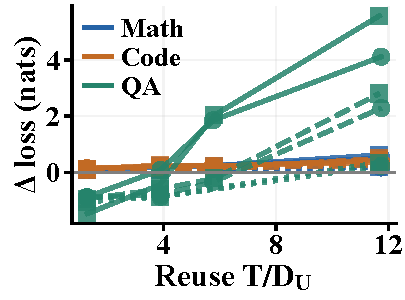
\includegraphics[width=\linewidth]{figs/fig1_a.pdf}\caption{Math}\label{fig:resp_a}\end{subfigure}\hfill
\begin{subfigure}[t]{1.35in}\centering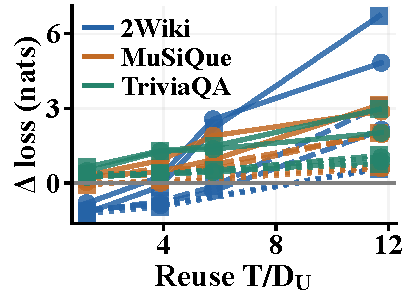
\includegraphics[width=\linewidth]{figs/fig1_b.pdf}\caption{Code}\label{fig:resp_b}\end{subfigure}\hfill
\begin{subfigure}[t]{1.35in}\centering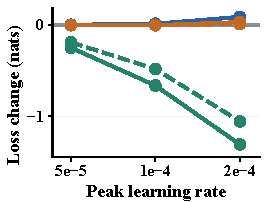
\includegraphics[width=\linewidth]{figs/fig1_c.pdf}\caption{QA on 2Wiki}\label{fig:resp_c}\end{subfigure}\hfill
\begin{subfigure}[t]{1.35in}\centering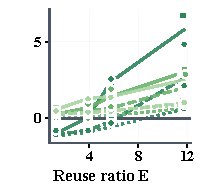
\includegraphics[width=\linewidth]{figs/fig1_d.pdf}\caption{QA, three distributions}\label{fig:resp_d}\end{subfigure}
\caption{Distillation transfer responses under one protocol: loss change in nats per native token from each student's initial state against the reuse ratio $E=T/D_U$ at the matched budget nearest 200k supervised tokens\rev{; dotted 270M, dashed 1B, solid 4B, markers the two pool seeds. Panel (d) rescores the same trajectories on a fresh 2Wiki sample, MuSiQue and TriviaQA.}}
\label{fig:responses_v2}
\end{figure}

\subsection{Pruning}
\label{sec:law_prune}

Mathematics and code share one density shape whose \rev{amplitude} depends on the model state
(Section~\ref{sec:state_config}), so we write their response as a state-dependent amplitude times a
\rev{shared density term},
\begin{equation}
\widehat{\Delta L}_c(\mathbf x,d)=A_c(\mathbf x)\,\Big(\frac{1-d}{0.3}\Big)^{\gamma_c},
\qquad
A_c(\mathbf x)=\beta_c\cdot\big(1,\tilde{\log N_0},\tilde L_{0,c},\tilde{\log D_0}\big),
\label{eq:power}
\end{equation}
with five parameters per capability and inputs standardized on the development set. \rev{Here $d$ is the retained density, so $1-d$ is the deleted fraction; $\gamma_c$ is a fitted exponent; the constant 0.3 sets the density coordinate so that the amplitude $A_c(\mathbf x)$ is the predicted loss change at $d=0.7$; and the tilde marks an input standardized with the mean and standard deviation of the development states, frozen at test time, so the four coefficients $\beta_c$ and $\gamma_c$ make five parameters. The shared density term pools information across checkpoints, and the amplitude reads only quantities available before compression.} Because the
density term is shared, a development grid can keep every state while measuring fewer densities per
state, and the validation target is the error at half the development measurements against the
full-grid regression on states in no fit (Section~\ref{sec:efficiency}). The form is fitted on Pythia
160M--1.4B at three pretraining stages over densities 0.6--0.9 and holds at new stages of sizes inside
that range; Appendix~\ref{sec:app_selbound} gives its selection among forms of the same complexity\rev{; on the measurement-efficiency confirmation, forms with the exponent fixed at one or replaced by a quadratic trail it by 0.04 to 0.20 nats and the pruning law of \citet{sengupta2025compression}, fitted on capability loss, by 0.04 to 0.06 on mathematics and code (Appendix Table~\ref{tab:a14-baselines})}. At sizes outside it, and for question answering, whose density response follows no
shared curve, the predictor is the pre-specified development median curve
$L_{0,c}+\widetilde f_c(d)$, which reads only the reference loss and which the selection rule of
Section~\ref{sec:selection} calls on every new \rev{model state and size}.

\subsection{Quantization}
\label{sec:law_quant}

Under quantization the response is a threshold in bit width whose position moves with the group size
(Section~\ref{sec:resp_capabilities}), so the predictors work on the measured configuration grid
rather than on a smooth surface. Per-channel quantization is predicted per bit width, by the per-bit
source regression on states in the fit and the per-bit median on new ones. Grouped quantization adds
the group size $g$ as a second axis: for mathematics and code on seen states the relation is a
piecewise interpolation over the measured $(b,g)$ grid, linear in $\log_2 g$, and otherwise it is the
per-configuration development median. Both are fitted on the Pythia states over 3--8 bits and groups
of 32--512 weights and validated at unseen group sizes of seen states and on a new state
(Section~\ref{sec:unseen_settings}). Here a complete description of the
configuration and coverage of its grid matter more than a parametric form, and the configuration
medians are the strong baseline that any quantization relation has to beat. \rev{The post-training-quantization law of \citet{kumar2024scaling}, exponential in precision with power laws in parameters and tokens, addresses the bit axis; its main form has no group-size axis, along which the 3-bit threshold moves here (Fig.~\ref{fig:pythia_responses}c), and refit on the same cells it is four to five times less accurate than the delivered relations for mathematics and code at unseen group sizes (Appendix~\ref{sec:app_kumar}).}

\subsection{Distillation}
\label{sec:law_distill}

Predicting the loss after distillation requires separating the amount of independent data, the
cumulative training exposure and the evaluation distribution (Section~\ref{sec:why}). The teacher
supplies the training targets and is fixed within the evaluated protocol, and the relations read
supervised completion tokens $T$, unique pool tokens $D_U$ and their ratio to predict the signed
transfer response of Section~\ref{sec:loss} as
\begin{equation}
\widehat\delta_c=a_c\log(1+E)\ (\text{math, code}),\qquad \widehat\delta_{\mathrm{QA}}=u\,(a+b\,u+q\,v),
\label{eq:kdforms}
\end{equation}
with $u=\log(1+T/T_{\mathrm{ref}})$ and $v=\log(D_U/D_{\mathrm{ref}})$ for reference constants fixed on
the development set: one parameter for mathematics and code, which vanish at zero budget, and three for question
answering. \rev{Here $T$, $D_U$ and $E=T/D_U$ are the supervised tokens, the unique pool tokens and the reuse ratio of Section~\ref{sec:why}; $a_c$ is the per-capability reuse coefficient; and $a$, $b$ and $q$ weight the budget, its square and the budget-pool interaction for question answering. The forms vanish at zero budget because an untrained student has no transfer response.} \rev{Leave-one-run-out comparison on the development runs selected these forms, a local approximation at the tested budgets and pools, since pre-specified structural checks neither reject nor establish an additive joint form (Appendix~\ref{sec:app_selbound}, Table~\ref{tab:distill_confirm}). The validation target is new pools and budgets of the Gemma-3 270M and 1B students under one recipe, with pools to 158k tokens, budgets of 50k--200k and question answering scored on 2Wiki (Section~\ref{sec:unseen_settings}); the 4B student and reuse near fourteen lie outside this domain.}
